\section{The study of human gut biodiversity through DNA}

Modern DNA sequencing technology has provided a way to read into the building blocks of life, from the first cultured bacteria to the first human genome \cite{Koonin1996-vp,Lander2001-vu}. Today, we only need a biological specimen with DNA to sequence and read the genetic blueprint to determine who is there. Before modern sequencing technology brought us this far, we had to differentiate between bacteria by looking at them under a microscope based on their morphology, thanks to the inventions of Van Leeuwenhoek \cite{Lane2015-yo}. Culturing techniques have further improved this method by allowing single-culture isolates. However, In a mixed biological sample from soil, ocean water or feces that contains thousands of different bacterial species, isolating, culturing and determining every single one is an impossible task \cite{Staley1985-zr}. As not all bacteria are obligate aerobic bacteria, but obligate anaerobes like the trillions of bacteria in the human gut, many would not survive culturing on a petri dish.\\

\noindent
A more precise determination of \textit{who} a bacteria is can be made through its genetic blueprint of the 16S ribosomal RNA gene \cite{Nr1985-yh}, which is an excellent phylogenetic marker for placing bacteria and archaea in the tree of life. The 16S rRNA gene is highly conserved between different bacteria and archaea due to its species specific signature of the letters A, T, C and G, which makes it useful for bacterial identification. Therefore, 16S rRNA sequencing technology has been an incredible tool for studying who is present in metagenomic samples from the human gut and allowed the first characterisations of commensal bacteria in the gut microbiome of hundreds of people. However, the metabolic and phenotypic traits of bacteria in an environment goes beyond the 16S rRNA marker gene. As a result, the desire to study the full genetic repertoire and \textit{what} bacteria can do within an environment lead to the advent of modern shotgun sequencing.

\section{Resolving uncultivated genomes in metagenomics}

Shotgun sequencing ushered in an era of genome-resolved metagenomics leading to the recovery of genes from novel uncultivated organisms \cite{Venter2004-ce}. Simultaneously, the popularity of metagenomics exploded as it became abundantly clear that the human microbiome is strongly correlated with health and markedly changed in disease states \cite{Lloyd-Price2016-qf}. High-throughput Illumina shotgun sequencing produces only short random fragments of DNA but in vast quantities. Powerful genome assembly algorithms were designed to utilize small repetitive sequence fragments to identify sequence overlaps and establish long continuous sequences, which were coined contigs. The strategies to resolve multiple uncultivated genomes from a random “soup” of contigs included (1) basic sequence alignment to a database of cultured sequence isolates (2) contig-binning based on similar GC-frequencies (3) tetranucleotide frequencies and (4) differential read-coverage. The read-coverage strategy (4) was based on the idea that contigs from the same genome should display a roughly similar sequencing depth. This data-driven strategy represented a powerful concept that many modern binners were later designed to leverage for binning genes or contigs into metagenomic assembled genomes (MAGs)\cite{Albertsen2013-en,Nielsen2014-vu,Kang2019-su}. The initial strategy used to determine when a MAG corresponded to a complete genome was based on the presence of essential bacterial single-copy genes (bacterial markers) \cite{Albertsen2013-en}, which is an approach still used to some extent today by bioinformatic tools like CheckM \cite{Parks2015-cs}.\\

\noindent
The presence of universal markers like the 16S rRNA gene and other single-copy gene markers in bacteria has enabled their identification in metagenomics and fuelled an explosion of known bacterial diversity during the last decades. Thus, the availability of bacterial genomic blueprints in the form of uncultivated bacterial genomes tallies hundreds of thousands across the human microbiome(s), ocean and soil \cite{Almeida2019-fk}. Meanwhile, the progress of developing databases containing genomes of other biotic constituents like fungi or viruses has been quite different. The reason why viruses were late to the party is due to several technical assembly challenges that will be addressed later, but most importantly they do not contain a universal virus marker gene. For the majority of people, viruses are considered obligate pathogens as we associate them to many types of diseases afflicted by human-infecting viruses, such as the Influenza virus. These types of viruses have represented the bulk of virus blueprints in databases for many years while the focus has been fixed on bacteria (Figure 1). As a result, most metagenomic sequences corresponding to an actual virus have resembled those in the current virus databases. From 2016 to 2018 (Figure \ref{fig:virushistory}) the number of uncultivated virus genomes exploded in the databases with 750,000 genomes when genomes mined from the first two large virus studies from ocean and soil were released \cite{Roux2016-yu,Paez-Espino2016-bb}. The success of these expansive viral studies could be attributed to the maturation of \textit{in vitro} protocols for concentrating viral particles, which enabled a greater space for viral assembly and identification.

\begin{figure}[H]
  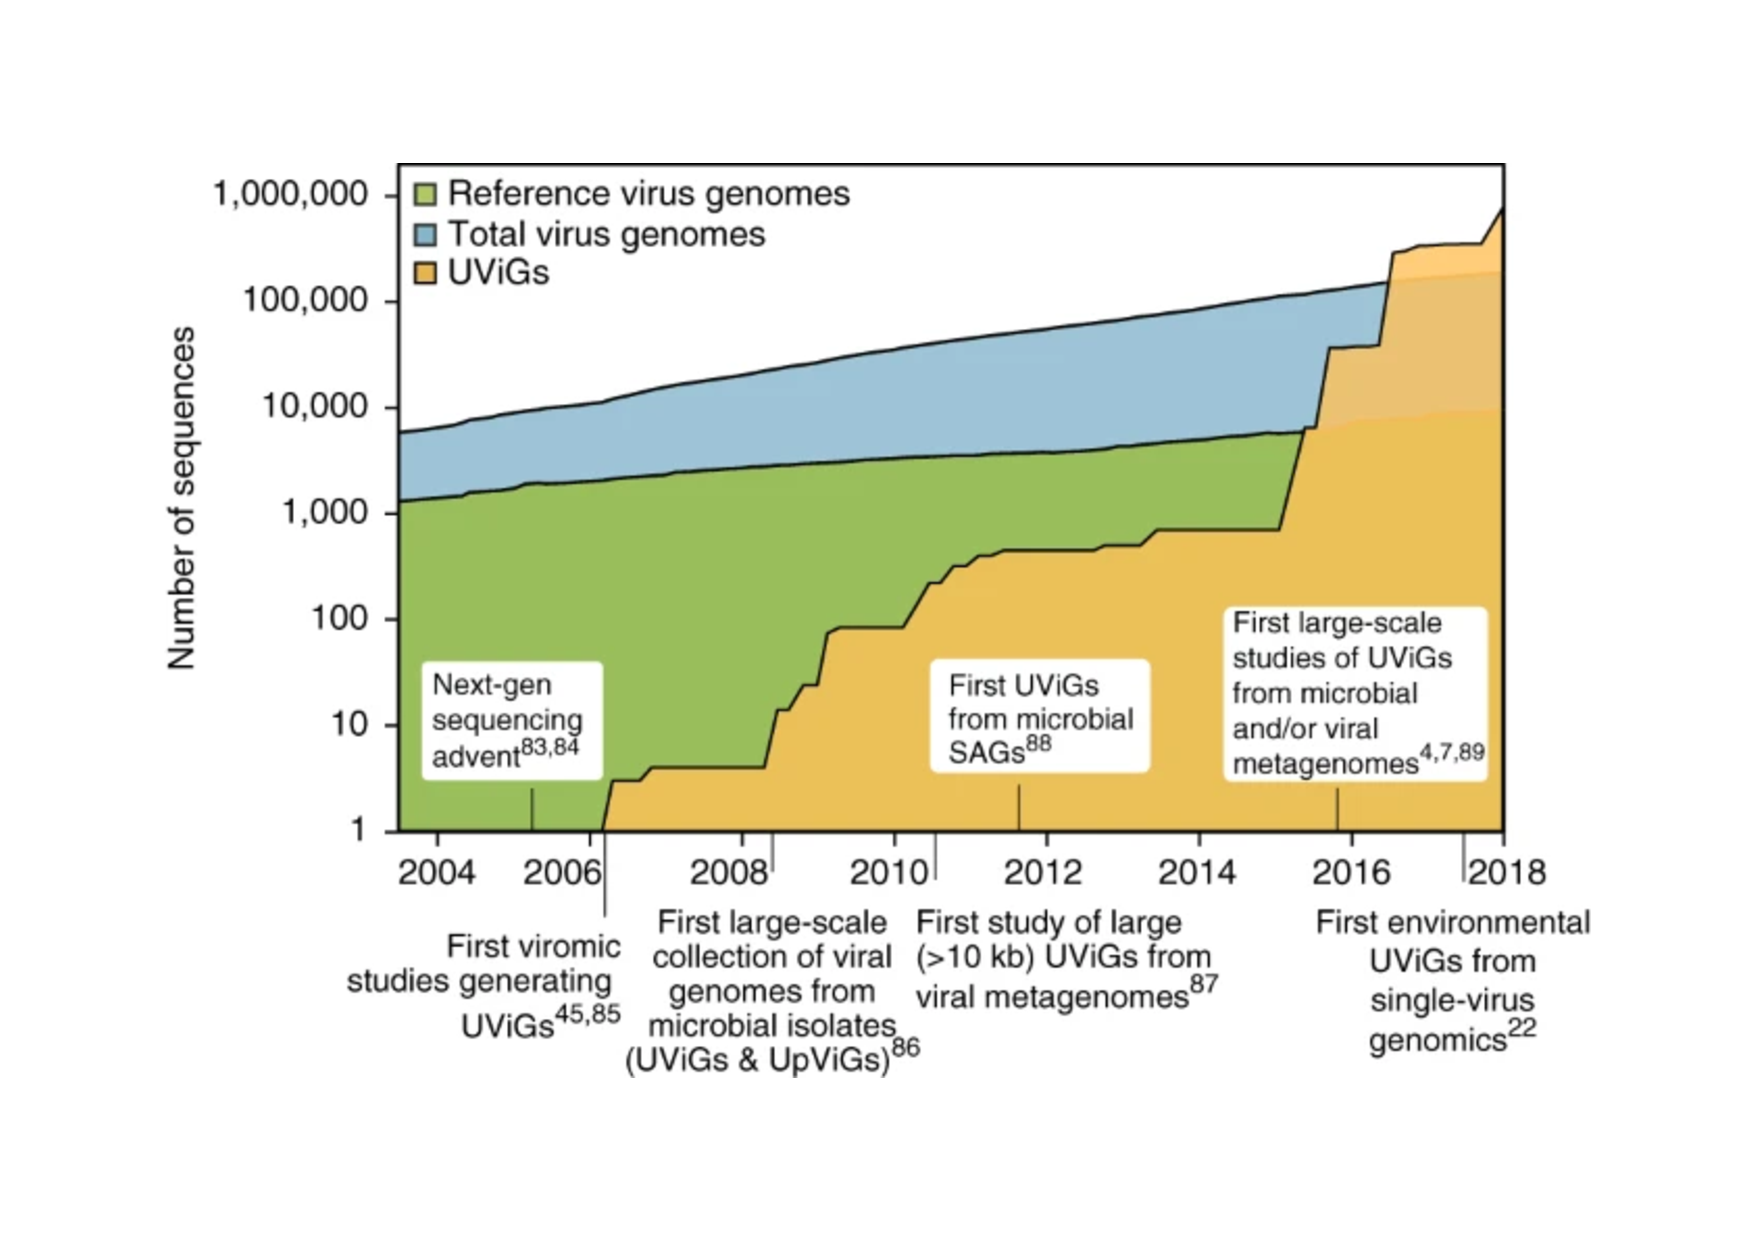
\includegraphics[scale=1, width=1\textwidth]{pictures/mroux2019.pdf}
  \caption[VirusTimeline]{The figure illustrates a recent timeline going back to 2004 and the cumulative number of virus genomes uploaded to genome databases since then, including uncultured virus genomes (UViGs). In addition, major events related to virus discovery are notated across the timeline. Virus genomes cultured \textit{in vitro} from isolates are depicted as blue and green, where the green corresponds to reference genomes at ncbi (\url{https://www.ncbi.nlm.nih.gov/nuccore}). The discovery of uncultured virus genomes (yellow) began in early 2006 and has since then exceeded the number of reference genomes many times over. Figure modified from \textit{Minimum Information about an Uncultivated Virus Genome} \cite{Roux2019-dc}.
  }
  \label{fig:virushistory}
\end{figure}

\noindent
We now recognise that virus particles can be identified almost anywhere where they sometimes massively outnumber other cells like bacteria \cite{Breitbart2018-sj}. To most people, it might be surprising that there are trillions of viral particles around us without the capacity to infect us as they prey on other microscopic organisms like bacteria. The group of viruses preying on bacteria are known as bacteriophages (phages for short). We are now recognising their impact and presence as early studies have unraveled a dynamic and changing virus community during disease like inflammatory bowel disease \cite{Norman2015-eb,Clooney2019-nn}. Therefore, the search for potential viral culprits has begun in addition to beneficial bacteriophages with protective properties. In order to understand how bacteriophages could be implicated in disease as they do not infect humans, we have to consider the way phages interact with bacteria who directly influence the human immune system and metabolism.